\clearpage

\section{Umsetzung Benchmark}\label{sec:ZigbeeUmsetzungBenchmark}
Die Umsetzung des Benchmarks geschah im Rahmen der Anforderungen des Benchmark Konzepts gemäss Abschnitt \ref{sec:BenchmarkKonzeptMeshNetzwerke}.
Wie im Abschnitt \ref{sec:Soft-undFirmware} bereits ausführlich behandelt wurde, sind innerhalb der Shared Library (siehe Abschnitt \ref{subsec:SharedLibrary}) klare Schnittstellen und Grenzen für die Mesh Protokollstacks definiert.
In den nachfolgenden Abschnitten wird auf die Umsetzung des Zigbee Stacks innerhalb dieser Grenzen eingegangen.

Das gesamte Zigbee Softwareprojekt ist im \href{https://github.com/Rouben94/P6_Software}{Github-Repository\footnote{\url{https://github.com/Rouben94/P6_Software}\cite{anklin_bobst_horath_rouben94p6_software_nodate}}} zu diesem Projekt unter dem Ordner \textbf{P6\_Software/Zigbee/zigbee\_benchmark/} abgelegt.
Darin enthalten ist je ein Projektordner für den \textit{Benchmark-Master}, \textit{Benchmark-Server} und \textit{Benchmark-Client}.
Ausserdem sind im Ordner \textbf{P6\_Software/Zigbee/zigbee\_benchmark/hex/} die vorkompilierten .hex Dateien abgelegt, welche direkt auf die nRF52840 SoC geflasht werden können. 

\subsection{Zigbee Software Development Kit}\label{subsec:ZigbeeSoftwareDevelopmentKit}
Für die Umsetzung von Zigbee Applikationen auf dem nRF52840 SoC stellt Nordic Semiconductor mit der \textit{nRF5 SDK for Thread and Zigbee\footnote{\url{https://www.nordicsemi.com/Software-and-tools/Software/nRF5-SDK-for-Thread-and-Zigbee}\cite{nordic_semi_nrf_sdk_for_thread_and_zigbee_2020}}} ein eigenes Software Development Kit (SDK) zur Verfügung.
Da Thread und Zigbee den gleichen \textit{IEEE 802.15.4} MAC Layer benutzen, teilen sich die beiden Protokollstacks eine gemeinsame SDK.
Innerhalb der SDK nutzen Thread und Zigbee jedoch unterschiedliche Ressourcen.

\begin{figure}[h]
	\centering
	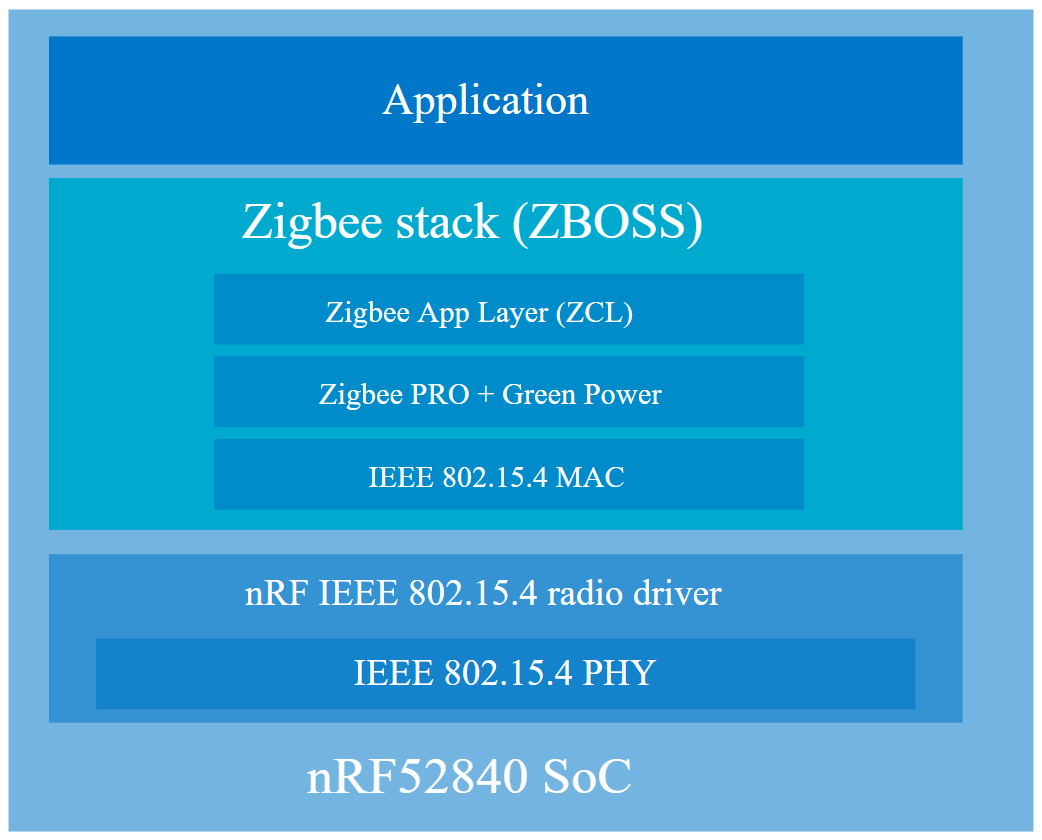
\includegraphics[width=0.6\textwidth]{Zigbee_SDK_Plattform_Design.png}
	\caption{nRF5 SDK for Thread and Zigbee Plattform Design Referenz für Zigbee Applikationen \cite{nordic_semi_nrf_sdk_for_thread_and_zigbee_2020}}
	\label{fig:ZigbeePlattformDesign}
\end{figure}

Für Zigbee Applikationen kommt ein Plattform Design gemäss Abbildung \ref{fig:ZigbeePlattformDesign} zum Einsatz. 
Als eigentlicher Zigbee Stack wird der \textit{ZBOSS} Zigbee Stack in der Version 3.3.0 von DSR\footnote{\url{https://dsr-iot.com/} \cite{dsr_corporation_dsr_nodate}} implementiert.
Dieser steht als vorkompilierte Library zur Verfügung. 
Es handelt sich dabei um einen weit verbreiteten \textit{Zigbee PRO} Stack, welcher die neuste Version der Zigbee Core Specification rev22 umsetzt.
\textit{ZBOSS} verwendet dabei ein kooperatives Multitasking Prinzip mit einem Scheduler, welcher die Tasks verwaltet.

Unter dem \textit{ZBOSS} Stack verwendet die SDK den \textit{nRF IEEE 802.15.4 radio driver} für die Ansteuerung der Funkschnittstelle.
Über dem \textit{ZBOSS} Stack befindet sich die Applikationsebene, in welcher Applikationen gemäss den ZCL Spezifikationen\footnote{\url{https://zigbeealliance.org/solution/zigbee} \cite{the_zigbee_alliance_zigbee_2016}} umgesetzt werden können.
\textit{ZBOSS} stellt die dafür notwendigen Funktionen zur Verfügung.


\subsection{Stack Implementation}\label{subsec:ZigbeeStackImplementation}
Der Zigbee Stack wurde mit Hilfe der \textit{nRF5 SDK for Thread and Zigbee}, wie oben beschrieben, implementiert.
Dazu mussten einige Punkte bei der Konzeptionierung und Umsetzung beachtet werden.
Diese Einzelheiten werden in den nächsten Abschnitten erläutert.

\subsubsection{Topologie}\label{subsubsec:ZigbeeTopologie}
Das Zigbee Netzwerk für den Benchmark wurde mit Hilfe des \textit{ZigBee PRO}-Stackprofils als vollständiges Mesh Netzwerk aufgebaut (siehe Abschnitt \ref{subsec:ZigbeeNetzaufbauundTopologie}).
Um dabei Resultate erhalten zu können, die mit jenen der beiden anderen Mesh Protokolle vergleichbar sind, wurden ausschliesslich \textit{Zigbee-Router} konfiguriert.
Total ergibt dies ein Mesh Netzwerk mit 50 \textit{Zigbee-Routern} und einem \textit{Zigbee-Koordinator}, welcher gleichzeitig ebenso als \textit{Zigbee-Router} fungiert.
Auf den Einsatz von \textit{Zigbee End-Devices} wurde verzichtet, da diese für die Performance des Netzes im gewählten Messkonzept (siehe Abschnitt \ref{sec:BenchmarkKonzeptMeshNetzwerke}) irrelevant sind.

\subsubsection{Wahl des Funkkanals}\label{subsubsec:FunkkanalWahlim2.4GHzISMBand}
Wie schon einige Male erwähnt, ist die Konkurrenz im 2.4GHz ISM Band gross.
Aus diesem Grund ist die Wahl des Funkkanals entscheidend für die Performance jedes Protokolls.
Zigbee respektive der \textit{IEEE 802.15.4} Standard bietet die Möglichkeit, den besten Funkkanal je nach Belastung automatisch zu bestimmen und auch während dem Betrieb zu ändern.
Dies bringt für den Benchmark jedoch einige Probleme, in Form von inkonstanten Bedingungen, mit sich.
Deshalb wurde der Funkkanal für das Zigbee Netzwerk in diesem Projekt fix hinterlegt.

\begin{figure}[h]
	\centering
	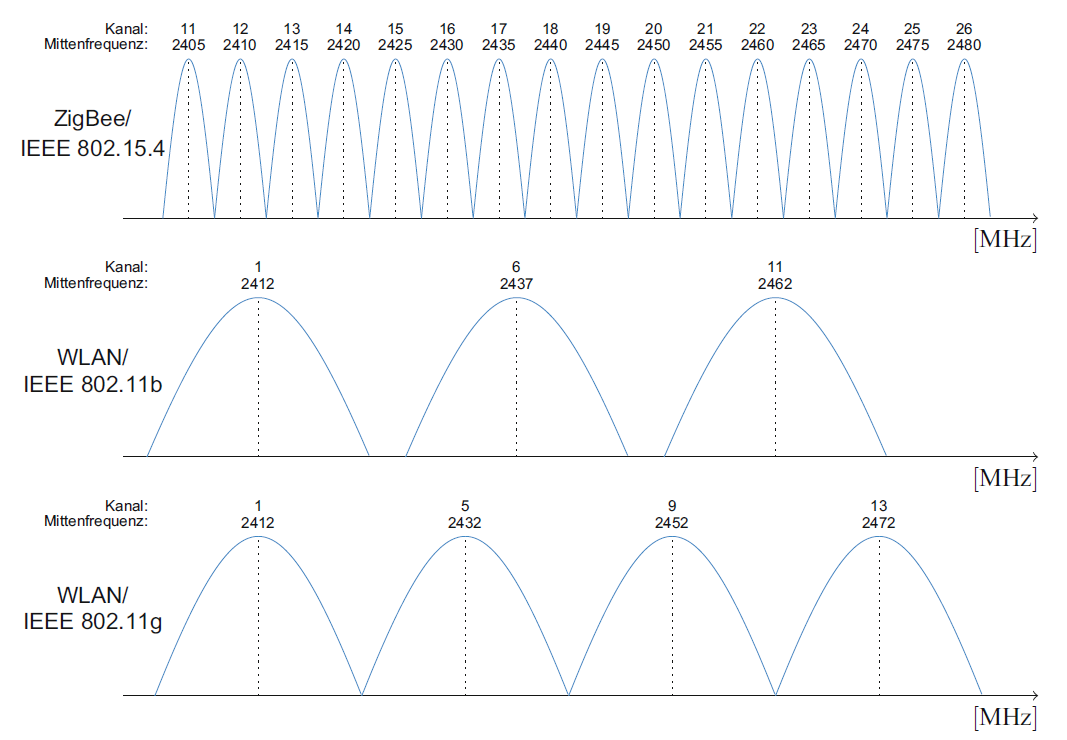
\includegraphics[width=0.7\textwidth]{Funkkanaele_Konkurrenz_IEEE.png}
	\caption{Konkurrenz Zigbee\slash IEEE und WLAN Funkkanäle \cite{markus_krause_rainer_konrad_drahtlose_2014}}
	\label{fig:ZigbeeKonkurrenzIEEEundWLANFunkkanaele}
\end{figure}

Abbildung \ref{fig:ZigbeeKonkurrenzIEEEundWLANFunkkanaele} zeigt, wie die Kanäle von \textit{Zigbee/IEEE 802.15.4} mit den WLAN Kanälen in Konkurrenz stehen.
Da in den Messumgebungen gemäss Abschnitt \ref{subsubsec:TestumgebungenundMessaufbau} eine störende Beinflussung durch WLAN Netze zu erwarten ist, wurde der Kanal 15 mit einer Mittenfrequenz von 2.425 GHz für die Benchmarks gewählt.
Dieser Kanal liegt genau zwischen den potentiell störenden WLAN Kanälen und wird daher am wenigsten beeinflusst.


\subsubsection{ZCL Level Cluster}\label{subsubsec:ZCLLevelCluster}
Der Performancevergleich der Mesh Protokolle soll gemäss Benchmark Konzept (siehe Abschnitt \ref{sec:BenchmarkKonzeptMeshNetzwerke}) auf Applikationsebene durchgeführt werden.
Wie im Abschnitt \ref{subsubsec:ApplicationLayer} beschrieben, wird die Applikationsebene gebildet durch die \textit{Zigbee Cluster Library (ZCL)}.
Für den Versand von Benchmark Nachrichten wurde deshalb der \textit{ZCL Level control cluster} implementiert.
Dieser definiert Attribute und Funktionen zur Steuerung eines Gerätes, welches einen Level Wert annehmen kann wie beispielsweise die Helligkeit einer dimmbaren Lampe.
Die verwendete SDK stellt den \textit{ZCL Level control cluster} standardmässig zur Verfügung.\cite{the_zigbee_alliance_zigbee_2016}


\subsubsection{Endpoint Handler}\label{subsubsec:EnpointHandler}
Der Empfang und die Verarbeitung von \textit{ZCL} Nachrichten wird in der \textit{nRF5 SDK for Thread and Zigbee} durch einen Callback Handler realisiert.
Dieser wird beim Start der Anwendung einmalig registriert und durch ein Callback-Ereignis der Radio Schnittstelle ausgelöst.
Im Zigbee Benchmark wurde ein \textit{Costum Endpoint Handler} implementiert, mit welchem die Benchmark Nachrichten ausgewertet werden können.
Nachrichten, welche an den \textit{Benchmark-Server-Endpoint} (siehe Abschnitt \ref{subsubsec:ApplicationLayer}) adressiert sind, werden in diesem Handler verarbeitet.
Die Registration des Handlers erfolgt durch den entsprechenden API Aufruf (siehe Abschnitt \ref{subsubsec:ZigbeeStackInitundKonfiguration}).

\subsubsection{APS Frame}\label{subsubsec:ZigbeeAPSFrame}
Während eines Benchmark Vorganges werden mit jeder Benchmark Nachricht die notwendigen Messgrössen gemäss Abschnitt \ref{subsec:VergleichswerteundMessgrössenMesh} generiert.
Dazu muss der \textit{Server Node}, also der Empfänger einer Nachricht, folgende Werte aus den Headern des Pakets auslesen:

\begin{itemize}
\item \textbf{Source Address:} \textit{Short-Address} des Senders
\item \textbf{Message ID:} Sequenznummer der empfangenen Benchmark Nachricht.
\end{itemize}

Diese Daten können dem APS Header des Pakets, welcher in Abbildung \ref{fig:AufbauAPSDatenframe} dargestellt ist, entnommen werden.
Die Message ID wird als \textit{uint\_16t}-Wert im \textit{Manufacturer Specific} Feld des erweiterten APS Header übermittelt.
Damit können 65535 Benchmark Nachrichten eindeutig identifiziert werden.
Die eigentliche Sequenznummer des ZCL Pakets ist nur ein \textit{uint\_8t}-Wert und kann deshalb nur bis zu einem Maximalwert von 255 inkrementiert werden.
Die Identifikation der Benchmark Nachrichten wäre somit aufwendiger.

\begin{figure}[h]
	\centering
	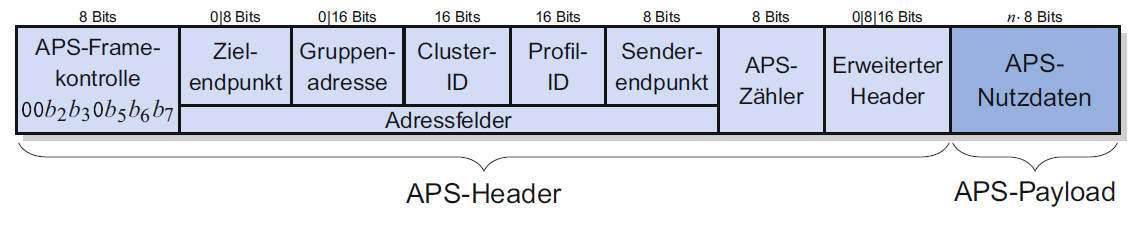
\includegraphics[width=0.8\textwidth]{Zigbee_APS_Datenframe.png}
	\caption{Aufbau APS Datenframe \cite{markus_krause_rainer_konrad_drahtlose_2014}}
	\label{fig:AufbauAPSDatenframe}
\end{figure}


\subsubsection{Adressierung}\label{subsubsec:Adressierung}
Die Adressierung der Nodes innerhalb des Zigbee Mesh Benchmarks kann entweder Unicast oder Multicast erfolgen.
Eine Multicast Adressierung wird mit Hilfe des \textit{ZCL Groups cluster} umgesetzt.
Dazu wird der Cluster auf den entsprechenden Nodes implementiert und diese werden mittels \textit{ZCL Add Group Request}-Befehl einer gewissen Gruppe hinzugefügt.
Eine solche Adressierung kann durch die Angabe einer \textit{Group Number} in der Konfiguration der Benchmark Nodes gemäss Abschnitt \ref{subsubsec:CLI} definiert werden.
Funktionstests zu Beginn der Benchmark Messungen haben allerdings gezeigt, dass diese Multicast Adressierung auf diesem Wege nicht praktikabel ist (siehe Abschnitt \ref{subsec:ZigbeeSchwierigkeitenbeiderUmsetzung}).
Deshalb wurden die Zigbee Benchmark Messungen im Unicast Modus durchgeführt.
Dabei werden die Benchmark Nachrichten direkt an die jeweiligen Empfänger gesendet.
Die Unicast Adressierung erfolgt durch Angabe der MAC Adressen der Empfänger bei der Konfiguration der Client Nodes (siehe Abschnitt \ref{subsubsec:CLI}).
Durch Abfrage der \textit{Adress-Tables} werden schliesslich die \textit{Short-Addresses} der Empfänger ermittelt.


\subsection{Mesh Node Firmware}\label{subsec:ZigbeeMeshNodeFirmware}
Die Firmware für die Benchmark Nodes, die in Abschnitt \ref{sec:Soft-undFirmware} bereits behandelt wurde, wird durch ein C- und ein H-Modul ergänzt, die spezifisch für die Implementation des Zigbee Stack zuständig sind.
Im Modul \textit{bm\_config.h} werden Konstanten für den Benchmark wie auch die Funktion des Stacks definiert.
Das Modul \textit{bm\_zigbee.c} hingegen beinhaltet je nach Funktion des Nodes (Master, Client oder Server) die entsprechenden Funktionen für die Initialisierung und Konfiguration des Stacks sowie das Benchmark Handling.
Darin ist der Versand und der Empfang der Benchmark Nachrichten vereint.
Der gesamte Sourcecode ist im \href{https://github.com/Rouben94/P6_Software}{Github-Repository\footnote{\url{https://github.com/Rouben94/P6_Software}\cite{anklin_bobst_horath_rouben94p6_software_nodate}}} zu diesem Projekt einsehbar.

\subsubsection{Stack Initialisierung und Konfiguration}\label{subsubsec:ZigbeeStackInitundKonfiguration}
Die Stack-Init-Routine wird durch die Benchmark Statemachine gemäss Abschnitt \ref{subsubsec:StatemachineSoftware} im State \textit{Init Benchmark} aufgerufen.
Diese Routine ist durch die Funktionen \textit{bm\_zigbee\_init()} und \textit{bm\_zigbee\_enable()} im Modul \textit{bm\_zigbee.c} abgebildet.
Hier wird der Zigbee Stack in der Rolle als \textit{Zigbee-Koordinator} resp. \textit{Zigbee-Server} initialisiert und hochgefahren.
Zudem wird auf dem \textit{Benchmark-Server} der Enpoint Handler gemäss Abschnitt \ref{subsubsec:EnpointHandler} mit dem folgenden API-Aufruf registriert:

ZB\_AF\_SET\_ENDPOINT\_HANDLER(BENCHMARK\_SERVER\_ENDPOINT,\linebreak bm\_ep\_handler)

Nach dem Start des Stacks wird der \textit{ZBOSS Mainloop} im Benchmark State abgearbeitet. Damit wird der \textit{ZBOSS Scheduler} aktiviert und der Stack wird ausgeführt.

Der \textit{Zigbee-Koordinator}, welcher auf dem Benchmark Master Node aufgesetzt ist, startet nun das \textit{Network Formation}, sofern keine persistenten Netzwerk Parameter gespeichert sind.
Dies ist nur beim Erststart des \textit{Benchmark-Masters} der Fall.
In der \textit{Network Formation} wird das Zigbee Netzwerk auf dem gewählten Kanal gebildet und die entsprechenden Netzwerkschlüssel generiert.
Ist beim Start eine persistente Konfiguration im Flash vorhanden, wird diese geladen und direkt mit dem \textit{Zigbee Commissioning} gestartet.
Ansonsten wird das erfolgreiche Beenden der \textit{Network Formation} abgewartet und erst danach das \textit{Zigbee Commissioning} gestartet.

Während dem \textit{Zigbee Commissioning} melden sich sämtliche Teilnehmer beim \textit{Zigbee-Koordinator} an und erhalten von diesem die nötigen Netzwerkparameter.
Unter anderem wird jedem Node eine 16-Bit \textit{Short-Address} zugewiesen.
Der Start des \textit{Commissioning} wird bei den Benchmark Teilnehmern um eine zufällige Zeit zwischen 0 und 30 Sekunden verzögert.
So kann sichergestellt werden, dass der \textit{Zigbee-Koordinator} nicht von gleichzeitigen Anfragen überhäuft wird.
Nach erfolgreichem \textit{Commissioning} ist das Zigbee Netzwerk bereit für die erste Messung.

Die gesamte \textit{Benchmark Init} Phase, wie sie im Abschnitt \ref{subsubsec:StatemachineSoftware} definiert wurde, ist auf die Dauer von 60 Sekunden limitiert.
Diese Zeit wird benötigt, um das \textit{Commissioning} abzuschliessen.
Danach wird automatisch in den \textit{Benchmark State} gewechselt.

\subsubsection{Benchmark Handling}\label{subsubsec:ZigbeeBenchmarkHandling}
Während der Master am Benchmark Handling nicht beteiligt ist,  sind im Modul \textit{bm\_zigbee.c} für den Benchmark Client und den Benchmark Server unterschiedliche Funktionen implementiert.
Im \href{https://github.com/Rouben94/P6_Software}{Github-Repository\footnote{\url{https://github.com/Rouben94/P6_Software}\cite{anklin_bobst_horath_rouben94p6_software_nodate}}} sind dafür die drei Projektdateien, \textit{benchmark\_master}, \textit{benchmark\_server} und \textit{benchmark\_client}, hinterlegt.

\paragraph{Benchmark Client}
Der Benchmark Client ist für den Versand von Benchmark Nachrichten zuständig.
Dazu wird durch die Benchmark-Statemachine, mittels universeller Schnittstelle in der SharedLib (siehe Abschnitt \ref{subsec:SharedLibrary}) die Funktion \textit{bm\_send\_message()} aufgerufen.
Diese Funktion löst wiederum einen Callback aus, in welchem die Benchmark Nachricht konstruiert und schliesslich versendet wird.
Die Nachricht ist einem \textit{ZCL Move to Level Request} nachempfunden.
Allerdings kann die Payload der Nachricht beliebig erhöht werden.

Noch vor dem Versand der Benchmark Nachricht werden die Message Infos in der Funktion \textit{bm\_read\_message\_info()} ausgelesen und ein Log-Eintrag wird erstellt.
Dabei handelt es sich um die Messgrössen gemäss Abschnitt \ref{subsec:VergleichswerteundMessgrössenMesh}.
Zudem wird der Zustand des grünen RGB-LEDs gewechselt.

\paragraph{Benchmark Server}
Der Benchmark Server wartet im \textit{Benchmark State} auf ankommende Nachrichten.
Sobald der Benchmark Server ein Paket empfängt, wird der Benchmark Endpoint Handler\linebreak \textit{(bm\_ep\_handler()} signalisiert.
Dieser entscheidet anhand der \textit{ZCL Cluster ID} ob es sich bei der Nachricht um eine Benchmark Nachricht handelt oder nicht.
Falls es sich um eine Benchmark Nachricht handelt, wird die Funktion \textit{bm\_receive\_message()} aufgerufen und die Referenz des Paket Buffers \textit{(bufid)} übergeben.
Mit Hilfe der \textit{bufid} werden nun die Message Infos ausgelesen und daraus ein Log Eintrag erstellt.
Zum Schluss wird der Status des blauen RGB-LED's gewechselt, womit der erfolgreiche Empfang einer Nachricht signalisiert wird.

\subsubsection{Benchmark und Stack Parameter}\label{subsubsec:BenchmarkundStackParameter}
Für die Umsetzung des Zigbee Protokollstacks sowie des Benchmark Frameworks für den Zigbee Benchmark mussten einige Parameter gesetzt oder neu definiert werden.
Die Tabelle \ref{tab:ZigbeeBenchmarkundStackParameter} zeigt die wichtigsten Benchmark- und Stack-Parameter.

\begin{table}[h]
\centering
\begin{adjustbox}{width=1\textwidth}
\begin{tabular}{|l|l|l|} 
\hline
Stack Init Time & 60000 ms & \begin{tabular}[c]{@{}l@{}}Zeit, die benötigt wird, um den Stack für den Benchmark\\zu initialisieren. \end{tabular} \\ 
\hline
Stack Startup max Delay & 30000 ms & \begin{tabular}[c]{@{}l@{}}Maximale Verzögerungszeit für den Startup des Zigbee Stacks\\auf allen Client und Server Nodes. Wird benötigt, um das Netz\\sauber aufbauen zu können.\end{tabular} \\ 
\hline
Network Formation Delay & 5000 ms & \begin{tabular}[c]{@{}l@{}}Zeit, die zur Stack Startup Delay Time addiert wird, um das\\Network Formation des Koordinators abzuwarten.\end{tabular} \\ 
\hline
\multicolumn{1}{l}{} & \multicolumn{1}{l}{} & \multicolumn{1}{l}{} \\ 
\hline
IEEE Channel & 15 & \begin{tabular}[c]{@{}l@{}}IEEE Kanal, der verwendet wird, um das Zigbee Mesh Netzwerk\\aufzubauen. \end{tabular} \\ 
\hline
Node Type & Zigbee-Router & Alle Nodes werden als Zigbee-Router konfiguriert \\ 
\hline
Client Endpoint & 1 & Nummer für den Client Endpoint im ZCL Level Cluster \\ 
\hline
Server Endpoint & 10 & Nummer für den Server Endpoint im ZCL Level Cluster \\ 
\hline
Default~Group ID & 0xB331 & \begin{tabular}[c]{@{}l@{}}Zu diesem Wert wird der Index für die zugewiesene Gruppe\\addiert, um damit die Gruppenzugehörigkeit festzulegen.\end{tabular} \\ 
\hline
\multicolumn{1}{l}{} & \multicolumn{1}{l}{} & \multicolumn{1}{l}{} \\ 
\hline
BSP LED 0 & ZIGBEE\_NETWORK\_STATE\_LED & Zeigt den Status der Netzwerkverbindung an. \\ 
\hline
BSP LED 1 & ERROR\_LED & Zeigt an, ob ein Fehler in der Statemachine vorliegt. \\ 
\hline
BSP LED 2 & CLIENT\_LED & \begin{tabular}[c]{@{}l@{}}Wird beim Versand einer Benchmark Nachricht ein oder\\ausgeschaltet.\end{tabular} \\ 
\hline
BSP LED 3 & BULB\_LED & \begin{tabular}[c]{@{}l@{}}Imitiert die Lichtquelle. Wird abwechselnd ein oder ausgeschaltet,~\\wenn ein Paket empfangen wird.\end{tabular} \\
\hline
\end{tabular}
\end{adjustbox}
\caption{Zigbee Benchmark- und Stack-Parameter}
\label{tab:ZigbeeBenchmarkundStackParameter}
\end{table}